\setlength{\parindent}{0pt}
\chapter{\bf DISCUSSION}

DNA replication is a highly conserved and regulated temporal process that is essential to genome inheritance. Yet, stochastic effects of DNA replication might cause mutagenesis contributing to cancer (Tomasetti \& Vogelstein, 2015). Therefore, an accurate and properly coordinated DNA replication is needed to prevent errors and to preserve DNA fidelity which is constantly threatened by both endogenous and exogenous sources during DNA replication. Considering 70,000 lesions occur in a single cell per day (Lindahl \& Barnes, 2000), DNA lesions must be removed before the next cell division, to avoid their permanent conversion into mutations. 

On the other hand, DNA excision repair mechanisms are known to relentlessly coup with DNA damages that are potential sites of mutations. In deficiencies of mismatch repair and nucleotide excision repair, there are specific mutational signatures associated which contribute to different cancer types (Helleday, Eshtad, \& Nik-Zainal, 2014). Nucleotide excision repair associated signature 7 displays replication timing differences and replication related strand asymmetry (Tomkova et al., 2018). Furthermore, because early replication domains are more reachable relative to late replication domains, mismatch repair causes a mutation difference between these domains by effectively repairing the mismatches at early replication domains (Supek \& Lehner, 2015). Similarly, TCR creates a transcriptional strand asymmetry by repairing adducts only at transcribed strands and leaving the opposite strand untouched (Zheng et al., 2014). Even though signature 7 is linked with DNA replication timing and strand asymmetry (Tomkova et al., 2018), the contribution of nucleotide excision repair to mutation differences during replication is still unclear. In this study, we performed Damage-seq and XR-seq methods on UV-irradiated HeLa cells that are synchronized at early and late S phases to quantify (6-4)PP and CPD damages and their repair events. 

\section{DNA replication elevates local nucleotide excision repair by mediating chromatin opening}

In the first part of the study, we examined the repair rate of nucleotide excision repair at large regions, while replication moves from early S phase to late S phase. To examine the repair rate on replication domains, we mapped damage and repair events to these regions. After calculating the repair rates, we found that ERD is repaired faster more efficiently that LRD. Because ERD usually corresponds to open chromatin sites, it is more reachable for nucleotide excision repair, in turn, promotes efficient repair. This result suggests that, like mismatch repair (Supek \& Lehner, 2015), nucleotide excision repair creates a mutational difference between ERD and LRD by efficiently repairing ERD. This phenomenon is less detectable for (6-4)PP damages than that of CPDs due to fast repair of (6-4)PPs.

Then, we examined the differences in repair rates of chromatin states for both ERD and LRD. The chromatin states that are associated with close regions are more varying in ERD, whereas the chromatin states that are associated with open regions displays same phenomenon in LRD, simply because ERD have less close regions, while LRD have less open regions. Expectedly, the active promoters and enhancers are repaired efficiently for both ERD and LRD. Moreover, the major difference between phases occurred on close chromatin states. This result indicates that movement of replication elevates the repair rates of close chromatin states by mediating chromatin opening. Lastly, we proposed a simple model to deminstrate the replication effect on repair (FIGUR).     

\begin{figure}[H]
    \begin{center}
    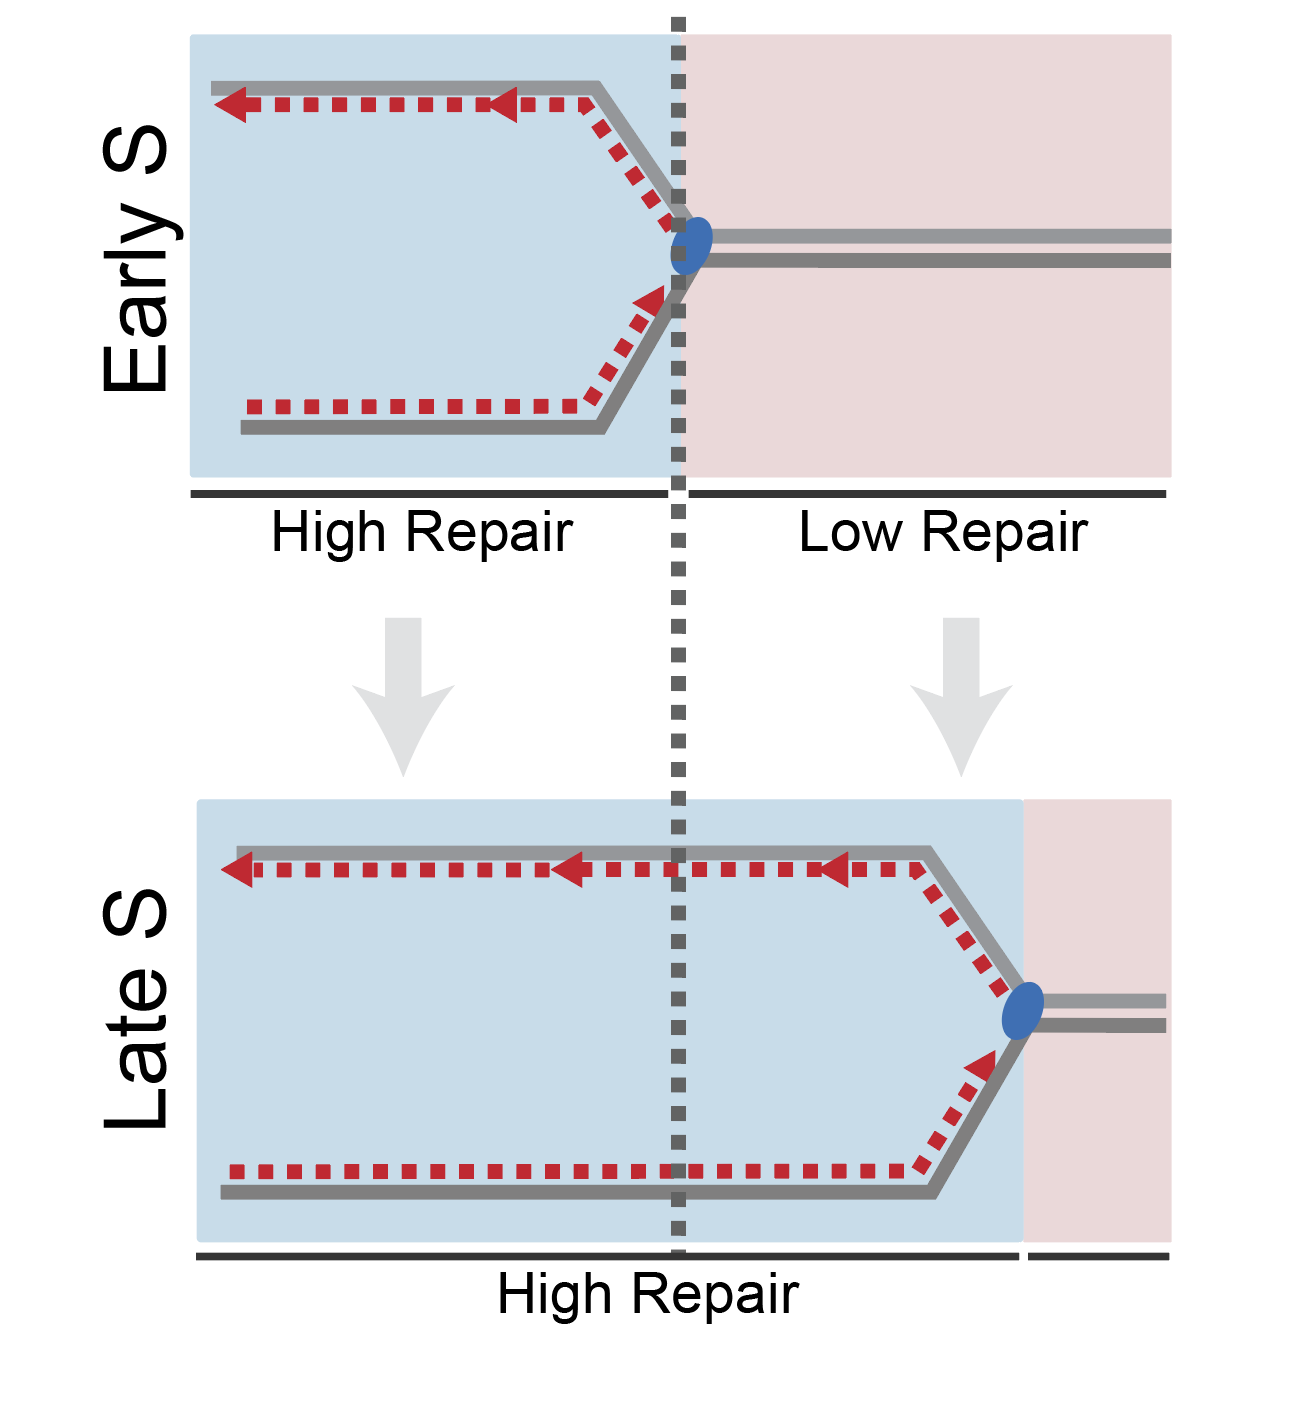
\includegraphics[width=\textwidth]{Chapters/5_discussion/figures/model}
    \caption[Repair preferences of Nucleotide Excision Repair during replication.]{Repair preferences of Nucleotide Excision Repair during replication. During the early S phase, open chromatin regions (blue) which mostly correspond to ERDs, are repaired better than the condensed regions (red) because excision repair can reach the open chromatin sites more efficiently than it reaches the condensed regions. While replication continues, those condensed regions loosen and become more reachable for excision repair.}
    \label{fig:model}
    \end{center}
    \end{figure}

\section{UV-induced DNA damage, repair and mutagenesis display replicational strand asymmetry}

Secondly, we examined a possible replicational strand asymmetry of mutagenesis, UV-induced DNA damage, and repair, respectively. After quantifying the melanoma mutations on initiation zones, we observed a significant mutational strand asymmetry that contains more mutations at lagging strands. Reasoning that this asymmetry around initiation zones should be related to nucleotide excision repair, we mapped damage and repair events on these regions separately. Remarkably, the same asymmetry was detectable for both damage and repair. Then, we simulated Damage-seq and XR-seq reads to see if the asymmetry is biased by the sequence context and the asymmetry was also detectable for the simulated reads. The results indicates that indeed the strand asymmetry around initiation zones are caused by the sequence context, initially at the level of UV-induced damages. Because there are more damages at lagging strands, repair also increases at lagging strand to cope with the damages. Conversely, when we normalized the repair with damage events, repair rates indicates an opposite asymmetry, higher repair rate at leading strands. These results suggest that even though repair events are higher at lagging strand due to high damages, the efficiency of repair elevates at leading strands, which also explains the less mutation counts at leading strands.         
